% Figura 2 — rede: VPC padrão da conta, as duas AZs do ALB, a subnet usada pelas
% três instâncias e a cadeia de security groups com a porta de cada salto.
\documentclass[11pt,tikz,border=6pt]{standalone}
\usepackage{fontspec}
\setmainfont{LibertinusSerif}[Extension=.otf, UprightFont=*-Regular,
  BoldFont=*-Bold, ItalicFont=*-Italic, BoldItalicFont=*-BoldItalic, Ligatures=TeX]
\setmonofont{Inconsolatazi4-Regular}[Extension=.otf, BoldFont=Inconsolatazi4-Bold,
  Ligatures=TeX, Scale=0.92]
\usetikzlibrary{arrows.meta,calc,shapes.geometric}

\definecolor{tinta}{HTML}{1F2933}
\definecolor{petroleo}{HTML}{0F766E}
\definecolor{ambar}{HTML}{B45309}
\definecolor{fundo}{HTML}{F5F7F8}

\begin{document}
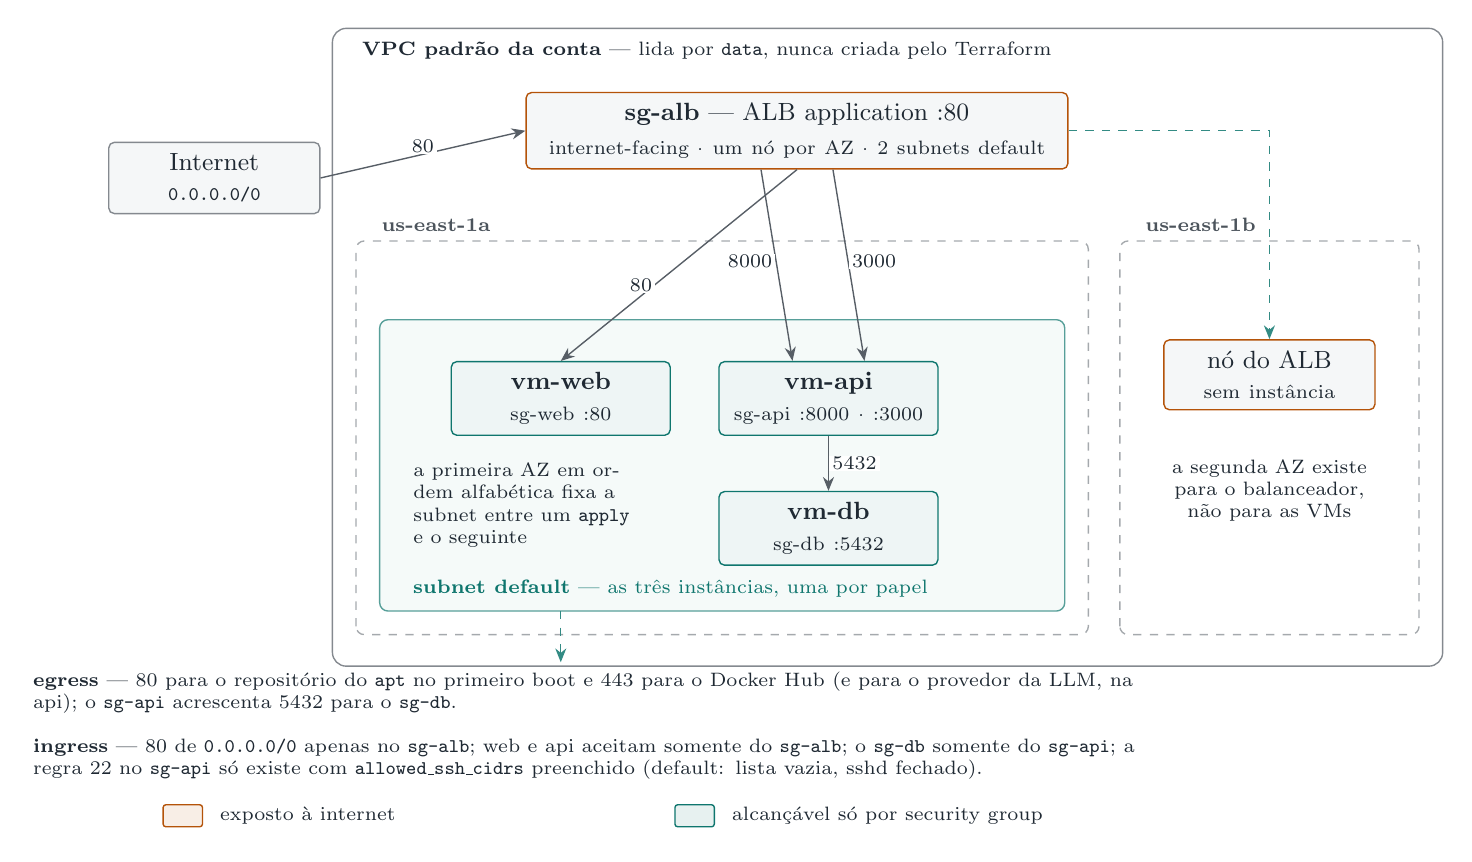
\begin{tikzpicture}[
    font=\small,
    >={Stealth[length=5pt,width=4pt]},
    pub/.style={draw=ambar, line width=0.5pt, fill=fundo, rounded corners=2pt,
      align=center, inner sep=4pt, text=tinta},
    priv/.style={draw=petroleo, line width=0.5pt, fill=petroleo!7, rounded corners=2pt,
      align=center, inner sep=4pt, text=tinta},
    ator/.style={draw=tinta!55, line width=0.5pt, fill=fundo, rounded corners=2pt,
      align=center, inner sep=4pt, text=tinta},
    nota/.style={align=left, inner sep=2pt, text=tinta, font=\scriptsize},
    seta/.style={->, line width=0.5pt, draw=tinta!75},
    ctrl/.style={->, dashed, line width=0.5pt, draw=petroleo!85},
    rot/.style={font=\scriptsize, text=tinta, fill=white, inner sep=1.2pt, inner ysep=0.5pt},
  ]

  % ---------- fora da conta ----------
  \node[ator, text width=2.4cm] (net) at (1.5,7.4)
    {Internet\\{\scriptsize \texttt{0.0.0.0/0}}};

  % ---------- VPC padrão ----------
  \draw[draw=tinta!55, line width=0.5pt, rounded corners=5pt]
    (3.0,1.2) rectangle (17.1,9.3);
  \node[nota, anchor=north west] at (3.3,9.2)
    {\textbf{VPC padrão da conta} — lida por \texttt{data}, nunca criada pelo Terraform};

  \node[pub, text width=6.6cm] (alb) at (8.9,8.0)
    {\textbf{sg-alb} — ALB application :80\\[1pt]
     {\scriptsize internet-facing · um nó por AZ · 2 subnets default}};

  % ---------- as duas AZs ----------
  \draw[draw=tinta!40, dashed, line width=0.5pt, rounded corners=3pt]
    (3.3,1.6) rectangle (12.6,6.6);
  \node[font=\scriptsize, text=tinta!80, anchor=south west] at (3.5,6.6)
    {\textbf{us-east-1a}};
  \draw[draw=tinta!40, dashed, line width=0.5pt, rounded corners=3pt]
    (13.0,1.6) rectangle (16.8,6.6);
  \node[font=\scriptsize, text=tinta!80, anchor=south west] at (13.2,6.6) {\textbf{us-east-1b}};

  \node[pub, text width=2.4cm] (no1b) at (14.9,4.9) {nó do ALB\\{\scriptsize sem instância}};
  \node[nota, anchor=north, text width=3.3cm, align=center] at (14.9,3.9)
    {a segunda AZ existe\\para o balanceador, não para as VMs};

  % ---------- a subnet usada ----------
  \draw[draw=petroleo!70, line width=0.5pt, rounded corners=3pt, fill=petroleo!4]
    (3.6,1.9) rectangle (12.3,5.6);
  \node[font=\scriptsize, text=petroleo, anchor=south west] at (3.9,1.95)
    {\textbf{subnet default} — as três instâncias, uma por papel};
  \node[nota, anchor=north west, text width=2.9cm] at (3.95,3.85)
    {a primeira AZ em ordem alfabética fixa a subnet entre um \texttt{apply} e o seguinte};

  \node[priv, text width=2.5cm] (web) at (5.9,4.6)
    {\textbf{vm-web}\\{\scriptsize sg-web :80}};
  \node[priv, text width=2.5cm] (api) at (9.3,4.6)
    {\textbf{vm-api}\\{\scriptsize sg-api :8000 · :3000}};
  \node[priv, text width=2.5cm] (db) at (9.3,2.95)
    {\textbf{vm-db}\\{\scriptsize sg-db :5432}};

  % ---------- arestas de tráfego ----------
  \draw[seta] (net.east) -- node[rot,above] {80} (alb.west);
  \draw[seta] (alb.south) -- node[rot,above left=-2pt,pos=0.62] {80} (web.north);
  \draw[seta] ([xshift=-13pt]alb.south) -- node[rot,left,pos=0.48] {8000} ([xshift=-13pt]api.north);
  \draw[seta] ([xshift=13pt]alb.south) -- node[rot,right,pos=0.48] {3000} ([xshift=13pt]api.north);
  \draw[seta] (api.south) -- node[rot,right] {5432} (db.north);
  \draw[ctrl] (alb.east) -- (14.9,8.0) -- (no1b.north);

  % ---------- saída ----------
  \draw[ctrl] (5.9,1.9) -- (5.9,1.25);
  \node[nota, anchor=north, text width=14.4cm] at (6.4,1.2)
    {\textbf{egress} — 80 para o repositório do \texttt{apt} no primeiro boot e 443 para o Docker Hub
     (e para o provedor da LLM, na api); o \texttt{sg-api} acrescenta 5432 para o \texttt{sg-db}.};
  \node[nota, anchor=north, text width=14.4cm] at (6.4,0.35)
    {\textbf{ingress} — 80 de \texttt{0.0.0.0/0} apenas no \texttt{sg-alb}; web e api aceitam somente
     do \texttt{sg-alb}; o \texttt{sg-db} somente do \texttt{sg-api}; a regra 22 no \texttt{sg-api}
     só existe com \texttt{allowed\_ssh\_cidrs} preenchido (default: lista vazia, sshd fechado).};

  % ---------- legenda ----------
  \node[draw=ambar, fill=ambar!10, minimum width=0.5cm, minimum height=0.28cm,
        line width=0.5pt, rounded corners=1pt] at (1.1,-0.7) {};
  \node[anchor=west, font=\scriptsize, text=tinta] at (1.45,-0.7) {exposto à internet};
  \node[draw=petroleo, fill=petroleo!10, minimum width=0.5cm, minimum height=0.28cm,
        line width=0.5pt, rounded corners=1pt] at (7.6,-0.7) {};
  \node[anchor=west, font=\scriptsize, text=tinta] at (7.95,-0.7)
    {alcançável só por security group};

\end{tikzpicture}
\end{document}
